%%%%%%%%%%%%%%%%%%%%%%%%%%%%%%%%%%%%%%%%%%%%%%%%%%%%%%%%%%%%%%%%%%%%%%%%%%%%%%%%
\begin{frame}[fragile]\frametitle{}
\begin{center}
{\Large Hugging Face}
\end{center}
\end{frame}

%%%%%%%%%%%%%%%%%%%%%%%%%%%%%%%%%%%%%%%%%%%%%%%%%%%%%%%%%%%
\begin{frame}[fragile]\frametitle{Who}
		\begin{itemize}
		\item Startup in New York, Paris and all over
		\item Started with Chatbots, social NLP
		\item But now, more famous as open-source model hub
		\item Transfer learning library: `Transformers'
		\end{itemize}
\end{frame}

%%%%%%%%%%%%%%%%%%%%%%%%%%%%%%%%%%%%%%%%%%%%%%%%%%%%%%%%%%%
\begin{frame}[fragile]\frametitle{Transformers}
		\begin{itemize}
		\item Easy to access SOTA (state of the art, latest-greatest) models
		\item All are based on ‘Transformer’ architecture
		\item Platform agnostic: Pytorch/TensorFlow/JAX
		\item Levels and usage:
				\begin{itemize}
				\item Researcher: Builds new models and makes them available here.
				\item Developer: Builds custom model on own dataset with programming
				\item User: Uses it as is for many tasks only in inference mode, not even with python
				\end{itemize}

		\end{itemize}
\end{frame}

%%%%%%%%%%%%%%%%%%%%%%%%%%%%%%%%%%%%%%%%%%%%%%%%%%%%%%%%%%%
\begin{frame}[fragile]\frametitle{Models}
			\begin{center}
			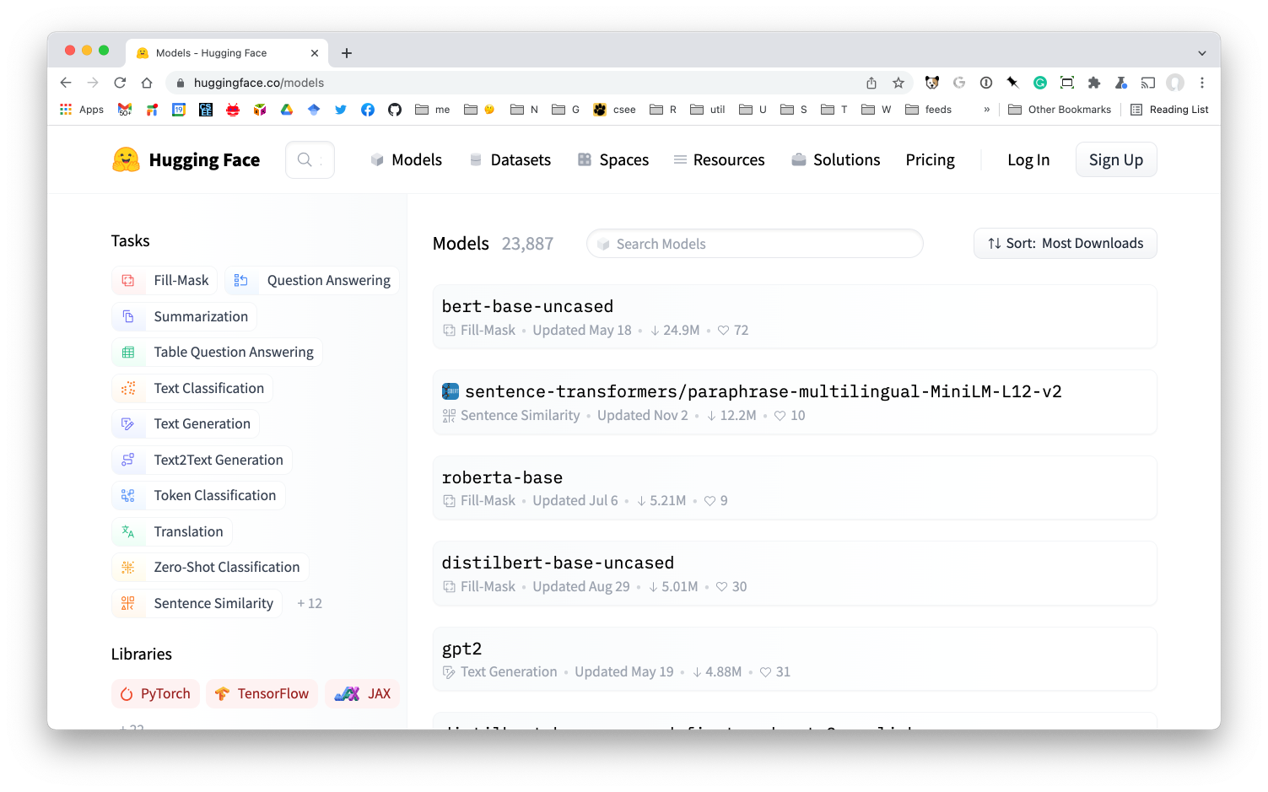
\includegraphics[width=\linewidth,keepaspectratio]{bert158}
			\end{center}	
\end{frame}

%%%%%%%%%%%%%%%%%%%%%%%%%%%%%%%%%%%%%%%%%%%%%%%%%%%%%%%%%%%
\begin{frame}[fragile]\frametitle{Same Interface}
			\begin{center}
			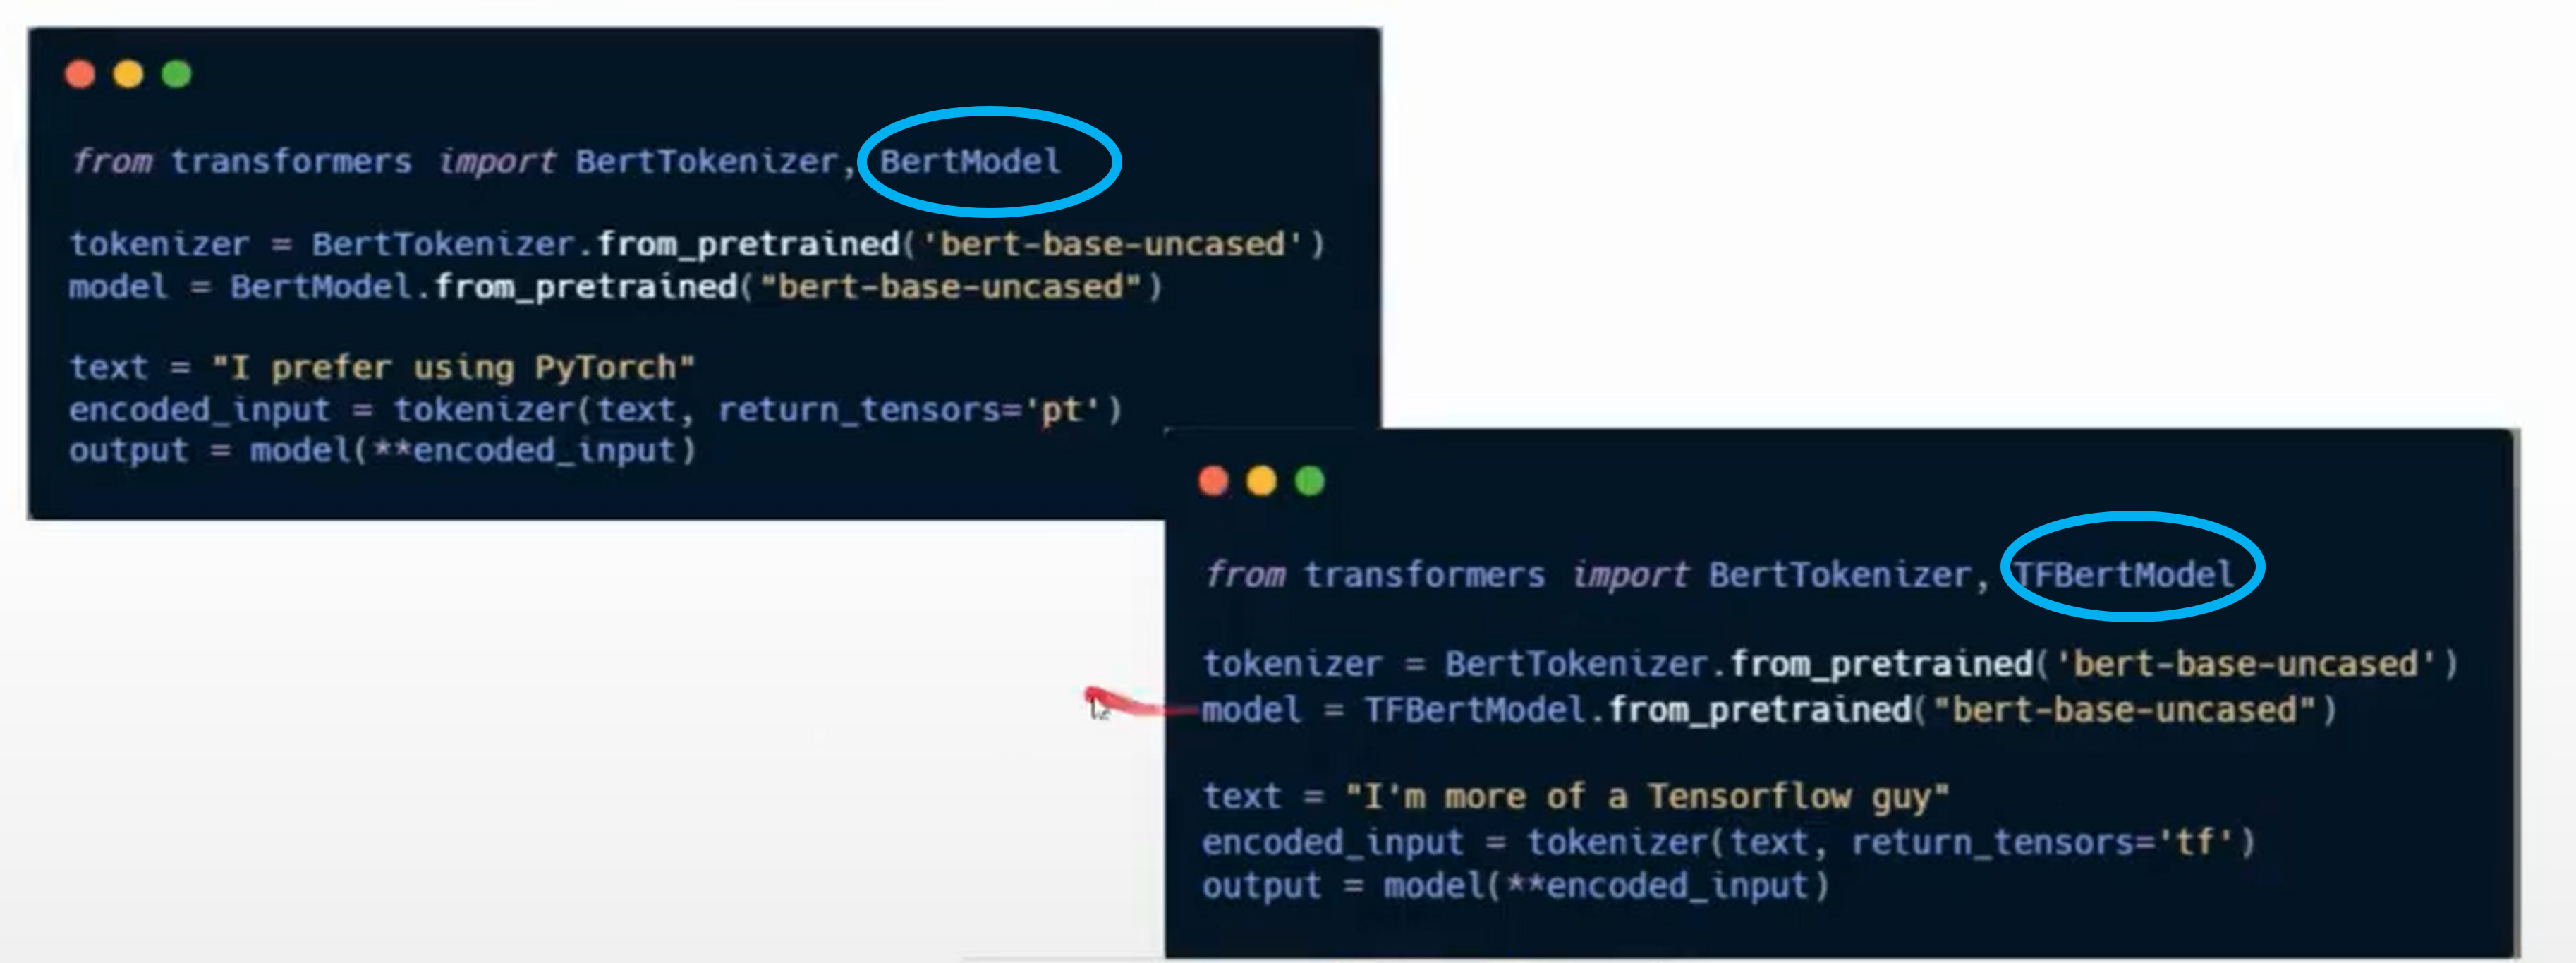
\includegraphics[width=\linewidth,keepaspectratio]{bert160}
			\end{center}	
\end{frame}

%%%%%%%%%%%%%%%%%%%%%%%%%%%%%%%%%%%%%%%%%%%%%%%%%%%%%%%%%%%
\begin{frame}[fragile]\frametitle{An overview of the Hugging Face Ecosystem}
			\begin{center}
			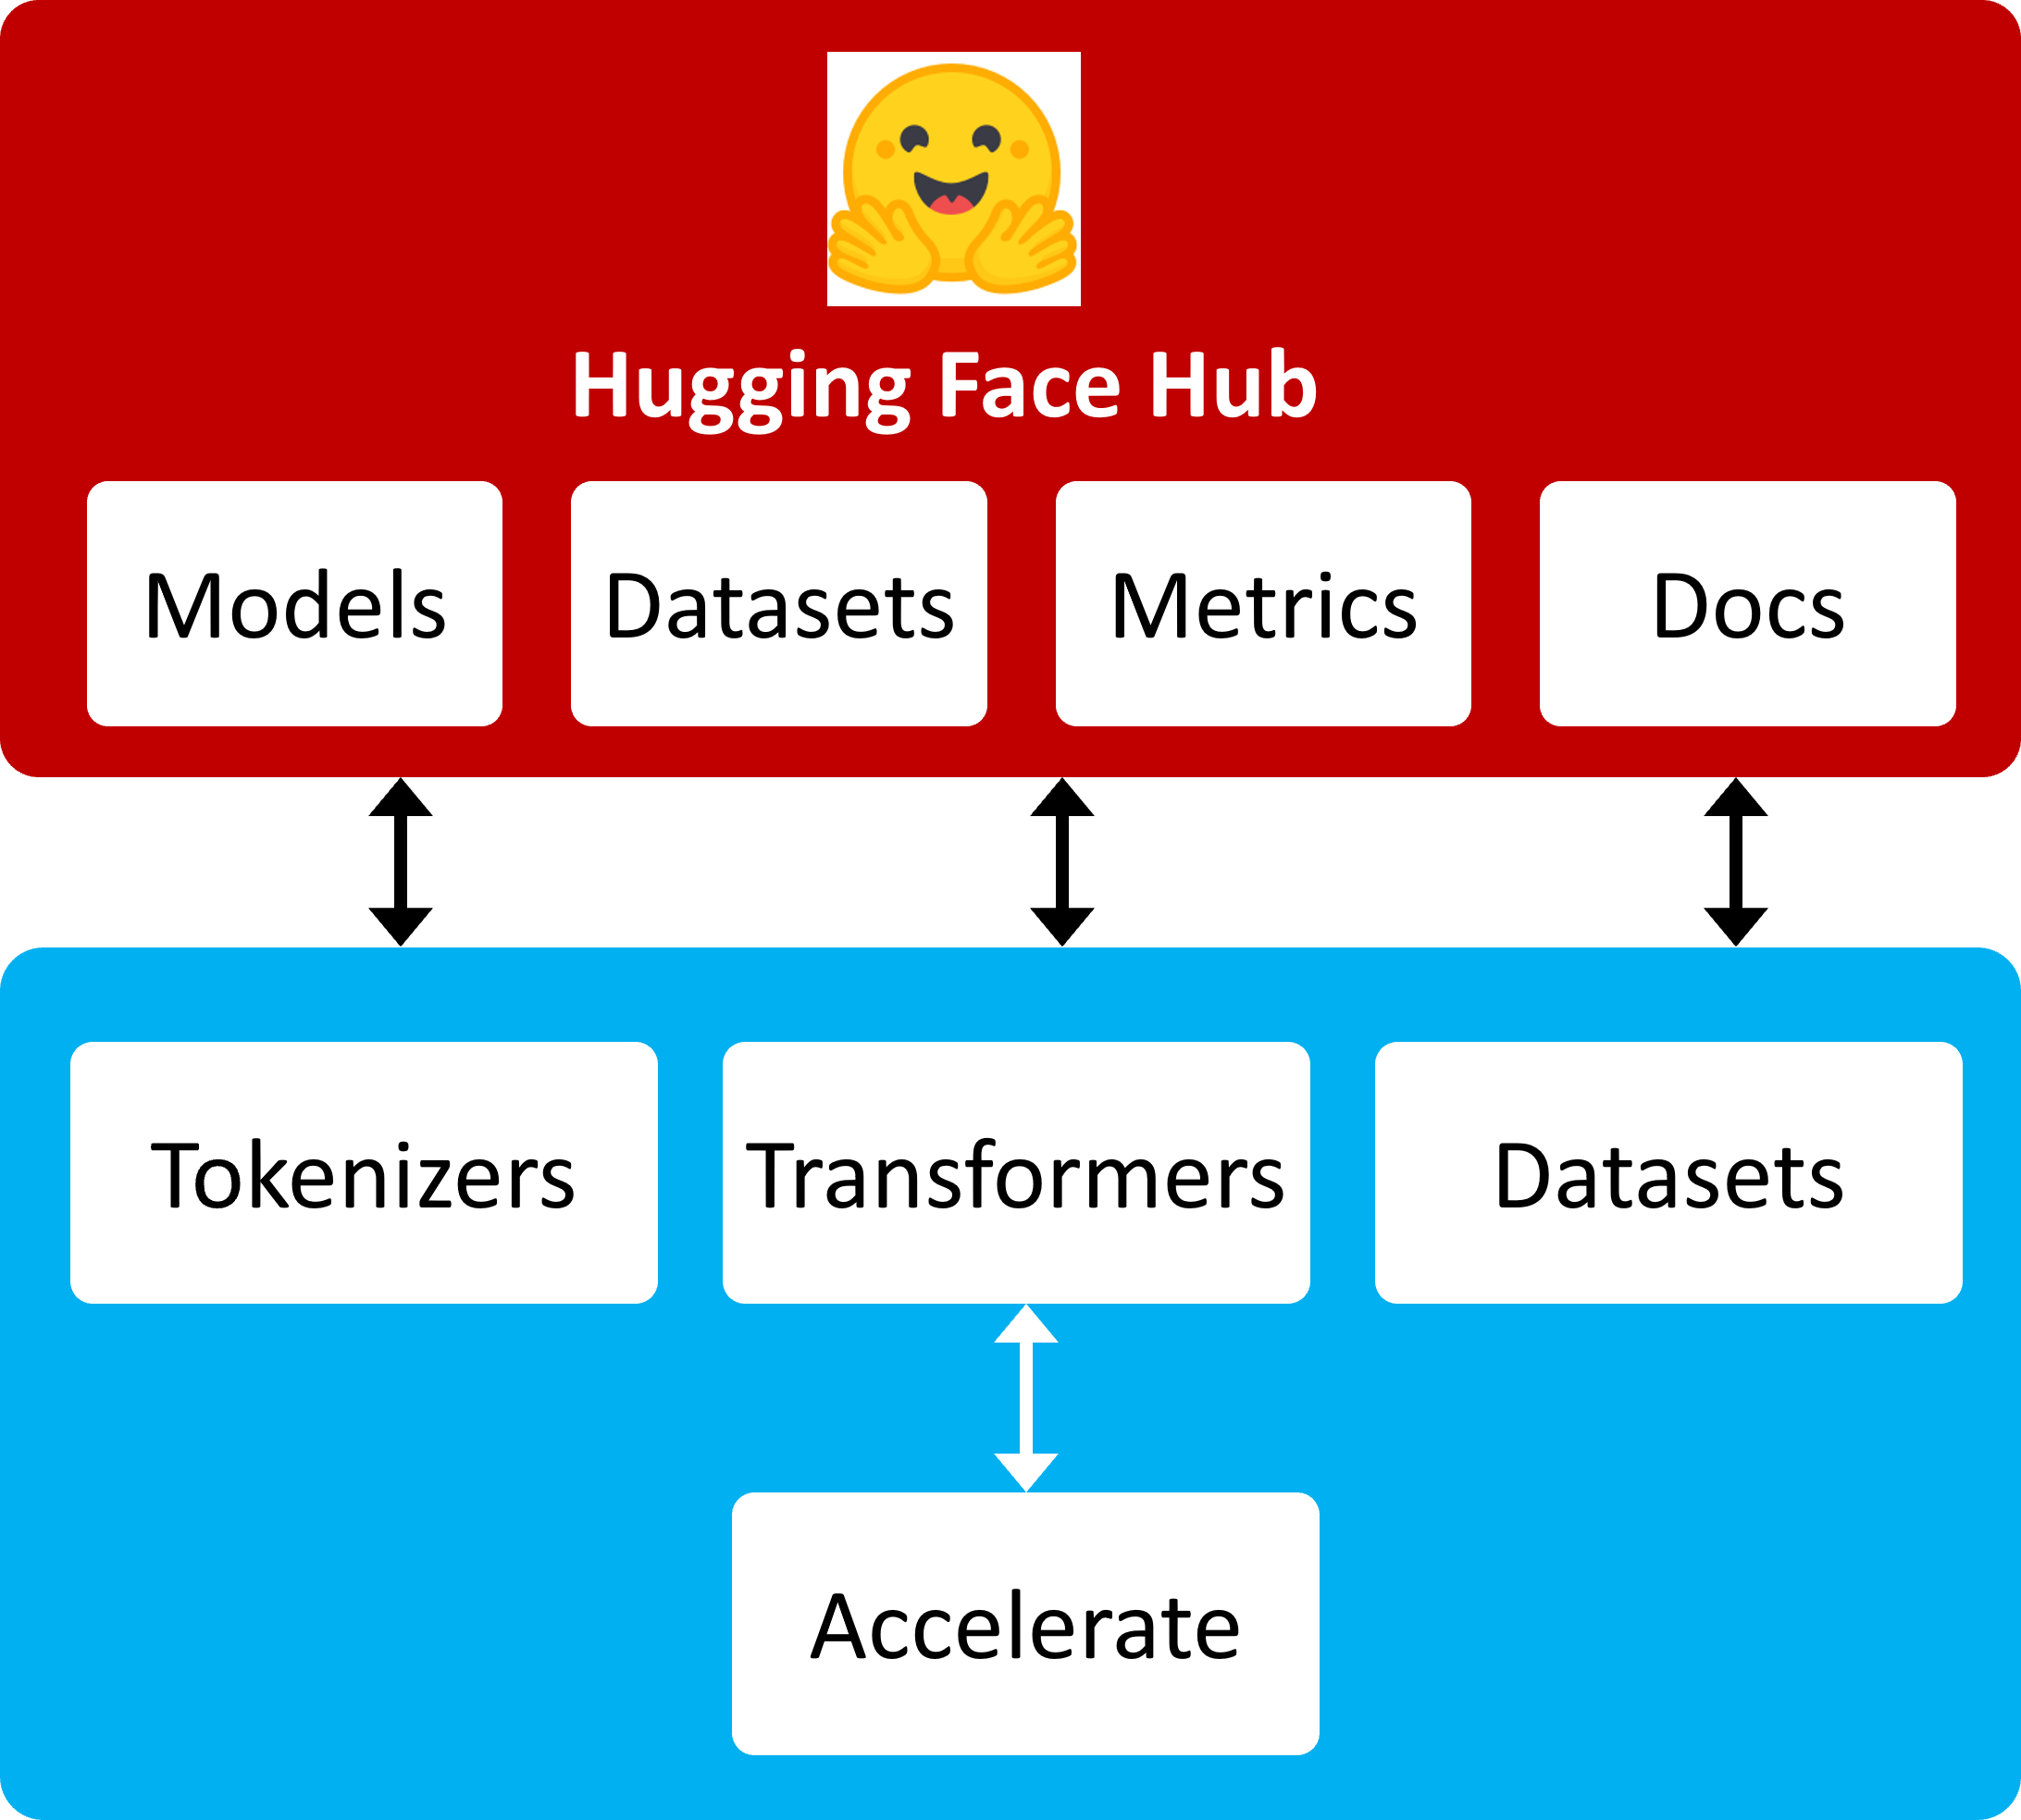
\includegraphics[width=0.6\linewidth,keepaspectratio]{bert161}
			\end{center}	
			
			% {\tiny (Source: Lewis Tunstall, Leandro von Werra, and Thomas Wolf (2022), Natural Language Processing with Transformers:  Building Language Applications with Hugging Face,  O'Reilly Media.)}
\end{frame}

%%%%%%%%%%%%%%%%%%%%%%%%%%%%%%%%%%%%%%%%%%%%%%%%%%%%%%%%%%%
\begin{frame}[fragile]\frametitle{A typical pipeline for training transformer models }

with the  Datasets,  Tokenizers, and  Transformers libraries

			\begin{center}
			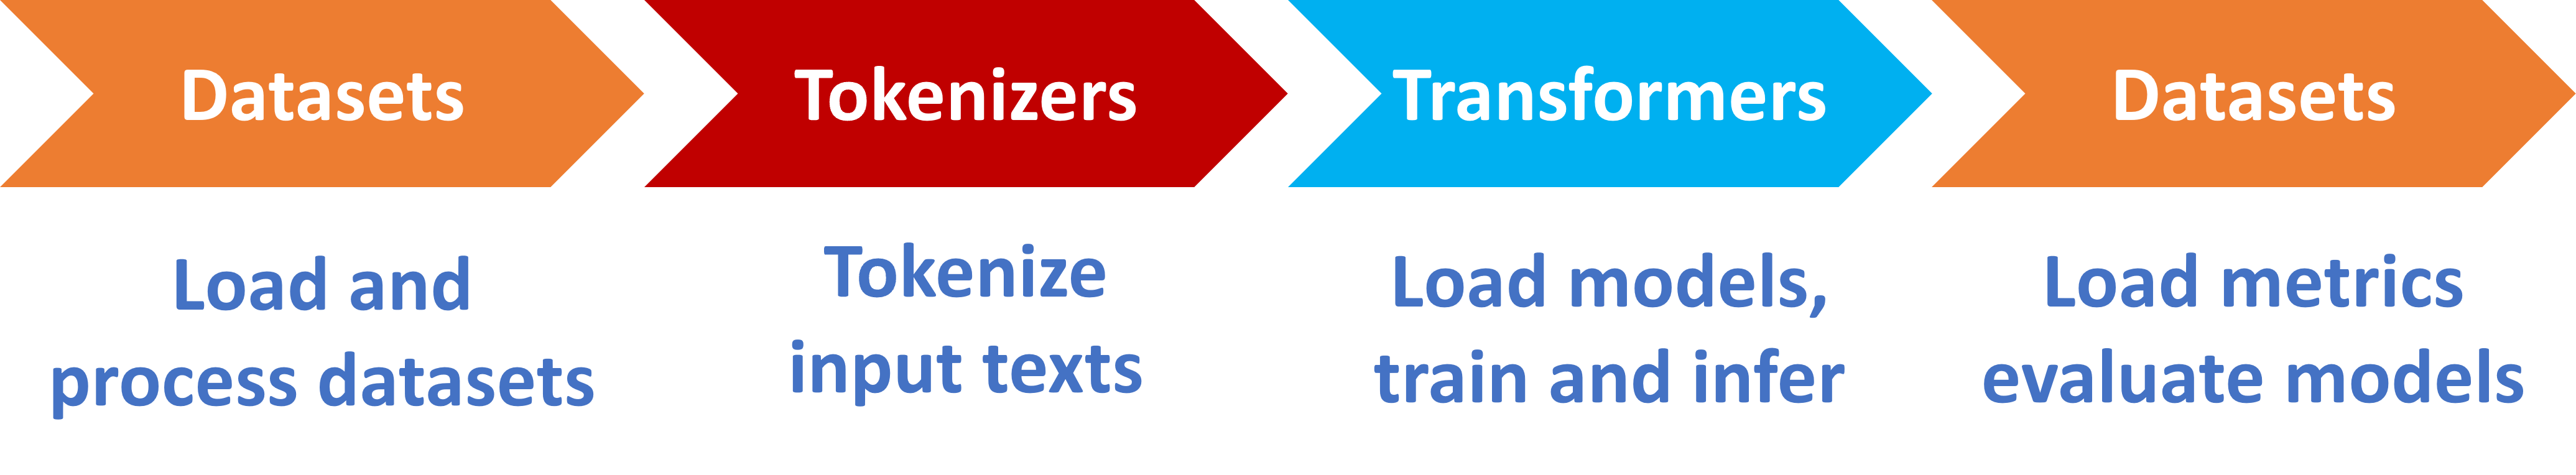
\includegraphics[width=\linewidth,keepaspectratio]{bert162}
			\end{center}	
			
			% {\tiny (Source: Lewis Tunstall, Leandro von Werra, and Thomas Wolf (2022), Natural Language Processing with Transformers:  Building Language Applications with Hugging Face,  O'Reilly Media.)}
\end{frame}

%%%%%%%%%%%%%%%%%%%%%%%%%%%%%%%%%%%%%%%%%%%%%%%%%%%%%%%%%%%
\begin{frame}[fragile]\frametitle{NLP with Transformers}

\begin{lstlisting}
!git clone https://github.com/nlp-with-transformers/notebooks.git
%cd notebooks
from install import *
install_requirements()

from utils import *
setup_chapter()
\end{lstlisting}
			
			% % {\tiny (Source: Lewis Tunstall, Leandro von Werra, and Thomas Wolf (2022), Natural Language Processing with Transformers:  Building Language Applications with Hugging Face,  O'Reilly Media.)}
\end{frame}

%%%%%%%%%%%%%%%%%%%%%%%%%%%%%%%%%%%%%%%%%%%%%%%%%%%%%%%%%%%
\begin{frame}[fragile]\frametitle{Text Classification}

\begin{lstlisting}
text = """Dear Amazon, last week I ordered an Optimus Prime action figure \
from your online store in Germany. Unfortunately, when I opened the package, \
I discovered to my horror that I had been sent an action figure of Megatron \
instead! As a lifelong enemy of the Decepticons, I hope you can understand my \
dilemma. To resolve the issue, I demand an exchange of Megatron for the \
Optimus Prime figure I ordered. Enclosed are copies of my records concerning \
this purchase. I expect to hear from you soon. Sincerely, Bumblebee."""
\end{lstlisting}
			
			% % {\tiny (Source: Lewis Tunstall, Leandro von Werra, and Thomas Wolf (2022), Natural Language Processing with Transformers:  Building Language Applications with Hugging Face,  O'Reilly Media.)}
\end{frame}

%%%%%%%%%%%%%%%%%%%%%%%%%%%%%%%%%%%%%%%%%%%%%%%%%%%%%%%%%%%
\begin{frame}[fragile]\frametitle{Text Classification}

			\begin{center}
			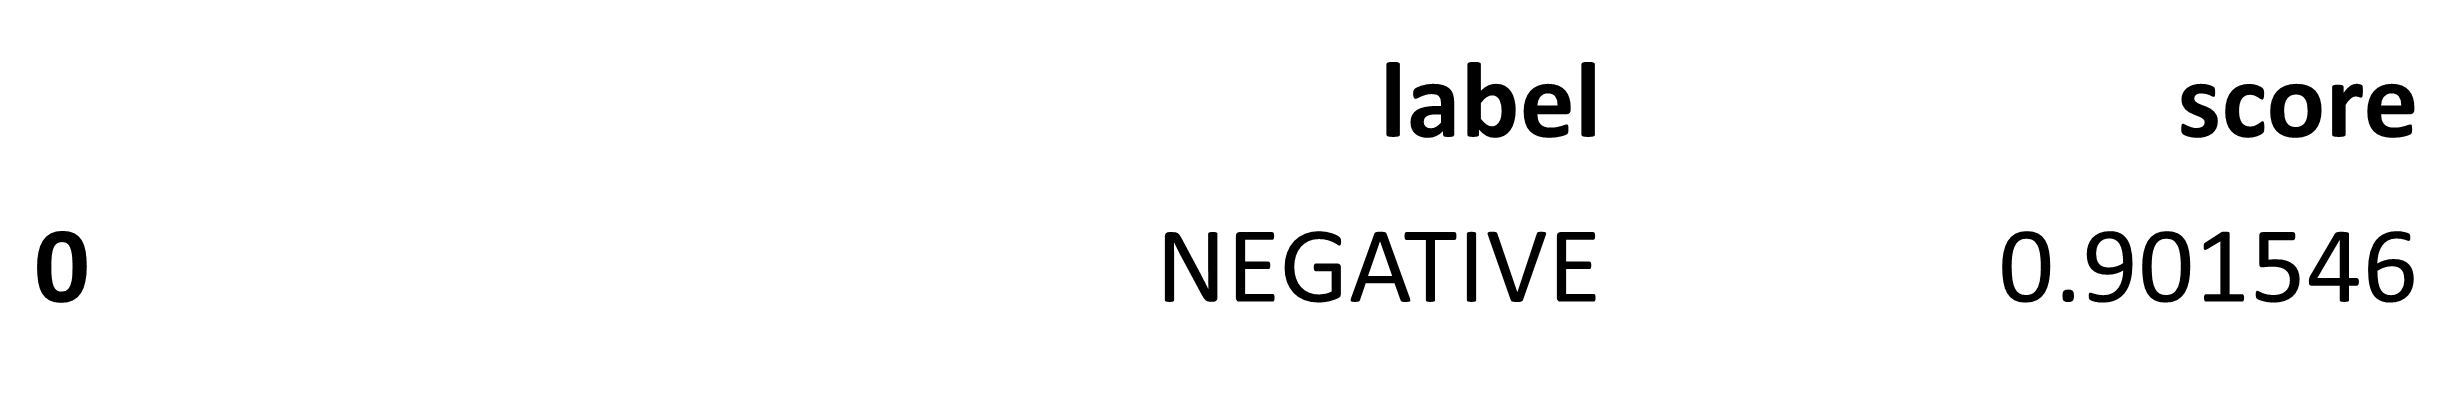
\includegraphics[width=0.5\linewidth,keepaspectratio]{bert163}
			\end{center}	
			
			
\begin{lstlisting}
from transformers import pipeline
classifier = pipeline("text-classification")

import pandas as pd
outputs = classifier(text)
pd.DataFrame(outputs) 
\end{lstlisting}
			
			

			
			% {\tiny (Source: Lewis Tunstall, Leandro von Werra, and Thomas Wolf (2022), Natural Language Processing with Transformers:  Building Language Applications with Hugging Face,  O'Reilly Media.)}
\end{frame}

%%%%%%%%%%%%%%%%%%%%%%%%%%%%%%%%%%%%%%%%%%%%%%%%%%%%%%%%%%%
\begin{frame}[fragile]\frametitle{Fine-Tuning Transformers Loading a pretrained model}

\begin{lstlisting}
from transformers import AutoModelForSequenceClassification
num_labels = 6
model = (AutoModelForSequenceClassification
.from_pretrained(model_ckpt, num_labels=num_labels)
.to(device))
\end{lstlisting}
			
			
			% % {\tiny (Source: Lewis Tunstall, Leandro von Werra, and Thomas Wolf (2022), Natural Language Processing with Transformers:  Building Language Applications with Hugging Face,  O'Reilly Media.)}
\end{frame}

%%%%%%%%%%%%%%%%%%%%%%%%%%%%%%%%%%%%%%%%%%%%%%%%%%%%%%%%%%%
\begin{frame}[fragile]\frametitle{Defining the performance metrics}

\begin{lstlisting}
from sklearn.metrics import accuracy_score, f1_score
def compute_metrics(pred):
	labels = pred.label_ids
	preds = pred.predictions.argmax(-1)
	f1 = f1_score(labels, preds, average="weighted")
	acc = accuracy_score(labels, preds)
	return {"accuracy": acc, "f1": f1}
\end{lstlisting}
			
			
			% % {\tiny (Source: Lewis Tunstall, Leandro von Werra, and Thomas Wolf (2022), Natural Language Processing with Transformers:  Building Language Applications with Hugging Face,  O'Reilly Media.)}
\end{frame}

%%%%%%%%%%%%%%%%%%%%%%%%%%%%%%%%%%%%%%%%%%%%%%%%%%%%%%%%%%%
\begin{frame}[fragile]\frametitle{Train the model}

\begin{lstlisting}
from huggingface_hub import notebook_login
notebook_login()
\end{lstlisting}
			
			
			% % {\tiny (Source: Lewis Tunstall, Leandro von Werra, and Thomas Wolf (2022), Natural Language Processing with Transformers:  Building Language Applications with Hugging Face,  O'Reilly Media.)}
\end{frame}

%%%%%%%%%%%%%%%%%%%%%%%%%%%%%%%%%%%%%%%%%%%%%%%%%%%%%%%%%%%
\begin{frame}[fragile]\frametitle{Train the model}

\begin{lstlisting}
from transformers import Trainer, TrainingArguments
batch_size = 64
logging_steps = len(emotions_encoded["train"]) // batch_size
model_name = f"{model_ckpt}-finetuned-emotion"
training_args = TrainingArguments(output_dir=model_name,
									num_train_epochs=2,
									learning_rate=2e-5,
									per_device_train_batch_size=batch_size,
									per_device_eval_batch_size=batch_size,
									weight_decay=0.01,
									evaluation_strategy="epoch",
									disable_tqdm=False,
									logging_steps=logging_steps,
									push_to_hub=True, 
									log_level="error")
\end{lstlisting}
			
			
			% % {\tiny (Source: Lewis Tunstall, Leandro von Werra, and Thomas Wolf (2022), Natural Language Processing with Transformers:  Building Language Applications with Hugging Face,  O'Reilly Media.)}
\end{frame}

%%%%%%%%%%%%%%%%%%%%%%%%%%%%%%%%%%%%%%%%%%%%%%%%%%%%%%%%%%%
\begin{frame}[fragile]\frametitle{Train the model}

\begin{lstlisting}
from transformers import Trainer
trainer = Trainer(model=model, args=training_args, 
						compute_metrics=compute_metrics,
						train_dataset=emotions_encoded["train"],
						eval_dataset=emotions_encoded["validation"],
						tokenizer=tokenizer)
trainer.train();
\end{lstlisting}
			
			\begin{center}
			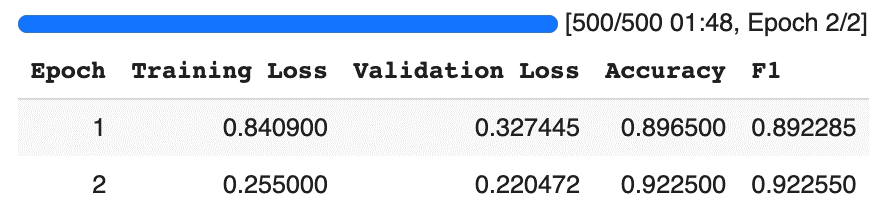
\includegraphics[width=0.5\linewidth,keepaspectratio]{bert164}
			\end{center}	
			
			% {\tiny (Source: Lewis Tunstall, Leandro von Werra, and Thomas Wolf (2022), Natural Language Processing with Transformers:  Building Language Applications with Hugging Face,  O'Reilly Media.)}
\end{frame}


%%%%%%%%%%%%%%%%%%%%%%%%%%%%%%%%%%%%%%%%%%%%%%%%%%%%%%%%%%%
\begin{frame}[fragile]\frametitle{Train the model}

\begin{lstlisting}
preds_output = trainer.predict(emotions_encoded["validation"])
preds_output.metrics
{'test_loss': 0.22047173976898193, 'test_accuracy': 0.9225, 'test_f1': 0.9225500751072866, 'test_runtime': 1.6357, 'test_samples_per_second': 1222.725, 'test_steps_per_second': 19.564}
y_preds = np.argmax(preds_output.predictions, axis=1)
plot_confusion_matrix(y_preds, y_valid, labels)
\end{lstlisting}
			

			
			% % {\tiny (Source: Lewis Tunstall, Leandro von Werra, and Thomas Wolf (2022), Natural Language Processing with Transformers:  Building Language Applications with Hugging Face,  O'Reilly Media.)}
\end{frame}

%%%%%%%%%%%%%%%%%%%%%%%%%%%%%%%%%%%%%%%%%%%%%%%%%%%%%%%%%%%
\begin{frame}[fragile]\frametitle{Fine-Tuning Transformers}

		
			\begin{center}
			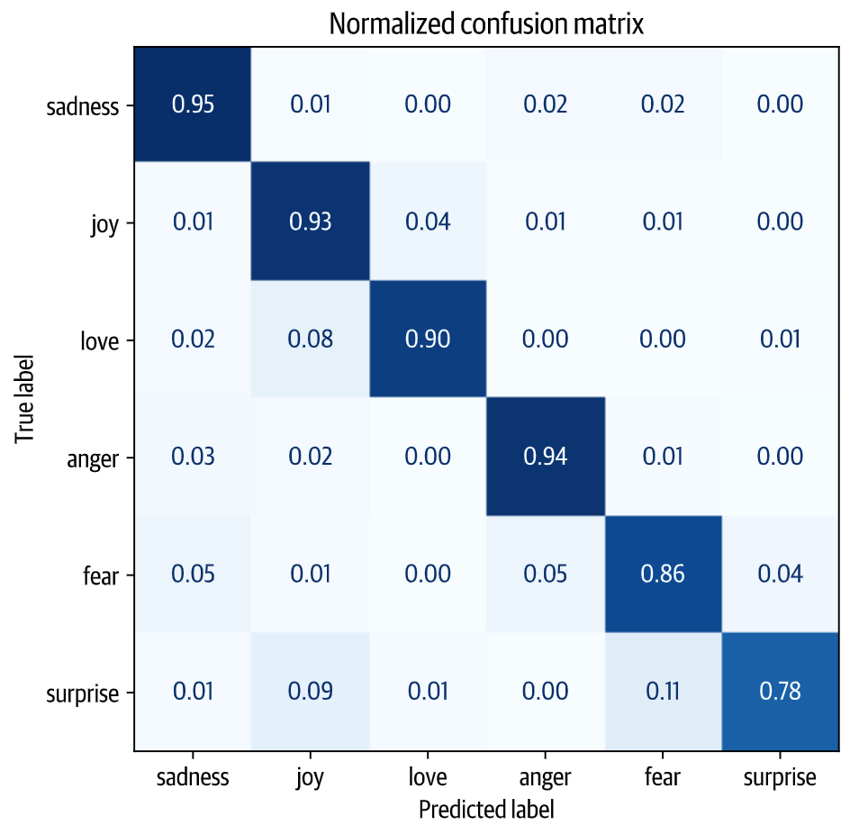
\includegraphics[width=0.5\linewidth,keepaspectratio]{bert165}
			\end{center}	
			
			% {\tiny (Source: Lewis Tunstall, Leandro von Werra, and Thomas Wolf (2022), Natural Language Processing with Transformers:  Building Language Applications with Hugging Face,  O'Reilly Media.)}
\end{frame}
